\documentclass[letterpaper,11pt,oneside,reqno]{article}

%%%%%%%%%%%%%%%%%%%%%%%%%%%%%%%%%%%%%%%%%%%%%%%%%%%%%%%%%%%%

\usepackage[pdftex,backref=page,colorlinks=true,linkcolor=blue,citecolor=red]{hyperref}
\usepackage[alphabetic,nobysame]{amsrefs}

%%%%%%%%%%%%%%%%%%%%%%%%%%%%%%%%%%%%%%%%%%%%%%%%%%%%%%%%%%%%
%main packages
\usepackage{amsmath,amssymb,amsthm,amsfonts,mathtools}
\usepackage{graphicx,color}
\usepackage{upgreek}
\usepackage[mathscr]{euscript}

%equations
\allowdisplaybreaks
\numberwithin{equation}{section}

%tikz
\usepackage{tikz}
\usetikzlibrary{shapes,arrows,positioning,decorations.markings}
\usepackage{pgfplots}
\pgfplotsset{compat=1.18}

%conveniences
\usepackage{array}
\usepackage{adjustbox}
\usepackage{cleveref}
\usepackage{enumerate}
\usepackage{datetime}

%paper geometry
\usepackage[DIV=12]{typearea}

%%%%%%%%%%%%%%%%%%%%%%%%%%%%%%%%%%%%%%%%%%%%%%%%%%%%%%%%%%%%
%draft-specific
\synctex=1
% \usepackage{refcheck,comment}

%%%%%%%%%%%%%%%%%%%%%%%%%%%%%%%%%%%%%%%%%%%%%%%%%%%%%%%%%%%%
%this paper specific
\newcommand{\ssp}{\hspace{1pt}}

%%%%%%%%%%%%%%%%%%%%%%%%%%%%%%%%%%%%%%%%%%%%%%%%%%%%%%%%%%%%
\newtheorem{proposition}{Proposition}[section]
\newtheorem{lemma}[proposition]{Lemma}
\newtheorem{corollary}[proposition]{Corollary}
\newtheorem{theorem}[proposition]{Theorem}
%%%%%%%%%%%%%%%%%%%%%%%%%%%%%%%%%%%%%%%%%%%%%%%%%%%%%%%%%%%%
\theoremstyle{definition}
\newtheorem{definition}[proposition]{Definition}
\newtheorem{remark}[proposition]{Remark}
%%%%%%%%%%%%%%%%%%%%%%%%%%%%%%%%%%%%%%%%%%%%%%%%%%%%%%%%%%%%

\begin{document}
\title{Lectures on Random Matrices
(Spring 2025)
\\Lecture 11: Asymptotics of Dyson Brownian Motion with an outlier}


\date{March 26, 2025\footnote{\href{https://lpetrov.cc/rmt25/}{\texttt{Course webpage}}
$\bullet$ \href{https://lpetrov.cc/simulations/model/random-matrices/}{\texttt{Live simulations}}
$\bullet$ \href{https://lpetrov.cc/rmt25/rmt25-notes/rmt2025-l11.tex}{\texttt{TeX Source}}
$\bullet$
Updated at \currenttime, \today}}



\author{Leonid Petrov}


\maketitle
\tableofcontents

\section{Recap}

\subsection{Dyson Brownian Motion (DBM)}
We introduced a time-dependent model of random matrices by letting an
\(N\times N\) Hermitian matrix \(\mathcal{M}(t)\) evolve in time so that each
off-diagonal entry follows independent Brownian increments (real or complex
depending on the symmetry class).  Setting
\[
\mathcal{M}(t) \;=\; \frac{1}{\sqrt{2}}\bigl(X(t) + X^\dagger(t)\bigr),
\]
where \(X(t)\) is an \(N\times N\) matrix of i.i.d.\ Brownian motions,
produces a self-adjoint matrix with a stochastically evolving spectrum.
This model is full-rank matrix Brownian motion,
and works well for $\beta=1,2,4$.
For other $\beta$, we need an SDE to describe the evolution of the eigenvalues (particles).

\subsection{Eigenvalue SDE}
Denote by \(\lambda_1(t)\ge\cdots\ge\lambda_N(t)\) the ordered eigenvalues of
\(\mathcal{M}(t)\).  Dyson showed that these eigenvalues form a
continuous-time Markov process satisfying the SDE
\[
d\lambda_i(t)
\;=\;
\frac{\beta}{2}\,\sum_{j\neq i}\,\frac{dt}{\lambda_i(t)-\lambda_j(t)}
\;+\;
dW_i(t),
\quad
i=1,\dots,N,
\]
where \(\beta>0\) and \(W_i(t)\) are independent standard real Brownian motions.
For classical random matrix ensembles (\(\beta=1,2,4\)), this SDE describes how
the eigenvalues evolve under real symmetric (GOE), Hermitian (GUE), or
quaternionic (GSE) Brownian motion --- in the last \href{https://lpetrov.cc/rmt25/rmt25-notes/rmt2025-l10.pdf}{Lecture 10} we discussed the cases \(\beta=1,2\) in detail.
A key feature is the \emph{repulsion} term
\(\frac{1}{\lambda_i-\lambda_j}\), which prevents collisions (and ensures the
ordering remains intact).

\subsection{Preservation of G\(\boldsymbol{\beta}\)E density}
A fundamental result is that starting from all eigenvalues at \(0\),
the distribution of \(\lambda(t)\) at time \(t\) has the joint density
proportional to
\[
\prod_{i<j}|\lambda_i - \lambda_j|^\beta\;
\exp\Bigl\{-\tfrac{1}{2t}\sum_i \lambda_i^2\Bigr\},
\]
matching the Gaussian \(\beta\)-Ensemble (G\(\beta\)E) law.  Hence DBM provides
a dynamical realization of G\(\beta\)E.  Invariance can be checked by verifying
that this density is annihilated by the generator of the SDE.

\subsection{Harish--Chandra--Itzykson--Zuber (HCIZ) integral}
The HCIZ integral is a key tool for computing matrix integrals involving traces.
For two Hermitian matrices \(A\) and \(B\) with eigenvalues
\((a_1,\dots,a_N)\) and \((b_1,\dots,b_N)\), it states (in one common
normalization):
\[
\int_{U(N)} \exp\bigl(\mathrm{Tr}(A\,U\,B\,U^\dagger)\bigr)\,dU
\;=\;
\prod_{k=1}^{N-1} k!\;
\frac{\det\bigl[e^{\,a_i b_j}\bigr]_{i,j=1}^N}{
\prod_{1\le i<j\le N}(a_j-a_i)\,\prod_{1\le i<j\le N}(b_j-b_i)}\,.
\]
This formula is instrumental in deriving transition densities for
\(\beta=2\) Dyson Brownian Motion.

\section{Optional: proof of HCIZ integral via representation theory}


In this section, we outline a standard argument (adapted from the theory of symmetric functions and representation theory of the unitary group) that leads to a proof of the Harish--Chandra--Itzykson--Zuber formula.  It is often referred to as the ``orbital integral'' or ``character expansion'' approach.

\smallskip

\noindent
\textbf{Step 1. Setting up the integral and Schur expansions.}
Let \(A\) and \(B\) be two \(N\times N\) diagonalizable matrices, with eigenvalues \(a_1,\ldots,a_N\) and \(\lambda_1,\ldots,\lambda_N\) respectively.  Denote by \(D_a = \mathrm{diag}(a_1,\ldots,a_N)\) and \(D_\lambda = \mathrm{diag}(\lambda_1,\ldots,\lambda_N)\).  We want to evaluate the integral
\[
I \;=\; \int_{U(N)} \exp\bigl(\mathrm{Tr}(D_a\,U\,D_\lambda\,U^\dagger)\bigr)\,dU
\]
over the Haar measure on \(U(N)\).

Since \(\mathrm{Tr}(B) = p_1(B)\) in the language of power sums
(where \(p_1(x_1,x_2,\dots) = x_1 + x_2 + \dots\)),
we have
\[
\exp\bigl(\mathrm{Tr}(B)\bigr) \;=\; \exp\bigl(p_1(B)\bigr).
\]
One can use a known expansion
\cite{Macdonald1995}
\[
e^{p_1(B)} \;=\;
\sum_{m=0}^{\infty} \frac{p_1^m(B)}{m!}
\;=\;
\sum_{m=0}^\infty \frac{1}{m!}\,
\sum_{\substack{\mu: |\mu|=m}}
\dim(\mu)\,s_\mu(B),
\]
where the sum is over all partitions \(\mu\) of size \(m\),
and \(s_\mu(\cdot)\) is the Schur polynomial (or Schur function) indexed by \(\mu\).  The coefficient \(\dim(\mu)\) is the dimension of the corresponding representation of \(S_m\).

We set \(B = D_a\,U\,D_\lambda\,U^\dagger\) and write
\[
I \;=\;
\int_{U(N)}
\exp\Bigl(\mathrm{Tr}(D_a\,U\,D_\lambda\,U^\dagger)\Bigr)\,dU
\;=\;
\int_{U(N)}
\sum_{m=0}^\infty
\frac{1}{m!}
\;\sum_{\substack{\mu:|\mu|=m}}
\dim(\mu)\;
s_\mu\bigl(D_a\,U\,D_\lambda\,U^\dagger\bigr)\,dU.
\]
One can exchange the integral and the sum (the series converges absolutely for all matrix arguments), giving
\begin{equation}
	\label{eq:HCIZ-I-start}
	I
	\;=\;
	\sum_{m=0}^\infty\;
	\sum_{\substack{\mu:|\mu|=m}}\;
	\frac{\dim(\mu)}{m!}
	\;\int_{U(N)} s_\mu(D_a\,U\,D_\lambda\,U^\dagger)\;dU.
\end{equation}

\smallskip

\noindent
\textbf{Step 2. Orthogonality of characters and the Unitary group.}
The Schur functions \(s_\mu(\cdot)\) can be seen as irreducible characters of the unitary group \(U(N)\) (up to a normalization factor) when restricted to \(N\)-tuples of eigenvalues.\footnote{$s_\mu$ for $\ell(\mu)\le N$ can be viewed as the character of the corresponding polynomial representation of $GL(N,\mathbb{C})$, then restricted to $U(N)$.  If $\ell(\mu) > N$, the function $s_\mu$ vanishes on $U(N)$. Thus,
we need to impose the condition \(|a_i|=|\lambda_i|=1\) (so that \(D_a,D_\lambda\in U(N)\)) to ensure immediate applicability of representation theory of $U(N)$, then extend to general \(\{a_i\}\) and \(\{\lambda_i\}\) by analytic continuation.}

\begin{proposition}[Functional equation for characters
	of compact groups]
	\label{prop:character-functional}
Let $G$ be a compact group with normalized Haar measure $dh$, and let $\chi$ be an irreducible character of a finite-dimensional representation of $G$. Then for any elements $g_1, g_2 \in G$, the following relation holds:
\begin{equation}
	\int_G \chi(g_1hg_2h^{-1})dh = \frac{\chi(g_1)\chi(g_2)}{\dim V},
\end{equation}
where $\dim V = \chi(e)$ is the dimension of the representation space.
\end{proposition}
\begin{remark}
	A similar relation holds for characters of finite groups.
\end{remark}
By \Cref{prop:character-functional}, the integral over $U(N)$ in \eqref{eq:HCIZ-I-start} can be evaluated as
\[
\int_{U(N)} s_\mu(D_a\,U\,D_\lambda\,U^\dagger)\,dU
\;=\;
\frac{1}{\mathrm{Dim}_N(\mu)}
\;s_\mu(a)\,s_\mu(\lambda),
\]
where
\(\mathrm{Dim}_N(\mu)\) is the dimension of the corresponding irreducible representation of $U(N)$.  Substituting back into \eqref{eq:HCIZ-I-start} yields
\[
I \;=\;
\sum_{m=0}^\infty\;
\sum_{\substack{\mu:|\mu|=m,\;\ell(\mu)\le N}}
\frac{\dim(\mu)}{m!}
\;\frac{1}{\mathrm{Dim}_N(\mu)}
\;s_\mu(a)\,s_\mu(\lambda),
\]
where \(\ell(\mu)\le N\) is needed for $s_\mu(\cdot)$ not to vanish on $U(N)$.

\smallskip

\noindent
\textbf{Step 3. Hook-length formulas and the final determinant.}
Next, one applies the hook-length formula
and the hook-content formula to dimensions:
\begin{equation*}
	\dim \mu=\frac{|\mu|!}{\prod_{\square\in\mu} h(\square)},
	\qquad
	\mathrm{Dim}_N(\mu)=\frac{\prod_{\square\in \mu}(N+c(\square))}{\prod_{\square\in\mu} h(\square)},
\end{equation*}
We have
\begin{equation*}
	\prod_{\square\in \mu}(N+c(\square))=\prod_{i=1}^{N}\frac{(\mu_i+N-i)!}{(N-i)!},
\end{equation*}
so identifying $m_i=\mu_i+N-i$ gives
\begin{equation*}
	I=0! 1! \cdots (N-1)!
	\sum_{m_1>\ldots>m_N\ge0 }\frac{s_\mu(a)s_\mu(\lambda)}{m_1!\cdots m_N!},
\end{equation*}
which yields the HCIZ formula by the Cauchy-Binet summation.

\section{Determinantal structure for $\beta=2$}

\subsection{Transition density}

\begin{theorem}[\(\beta=2\) Dyson Brownian Motion Transition Probabilities]
	\label{thm:dbm-transition}
For \(\beta=2\), let \(\lambda(t)=(\lambda_1(t)\ge \cdots \ge \lambda_N(t))\) follow Dyson Brownian Motion starting at \(\lambda(0)=\mathbf{a}=(a_1\ge \cdots \ge a_N)\).  Then for each fixed time \(t>0\),
\[
P\bigl(\lambda(t) = \mathbf{x}\;\big|\;\lambda(0)=\mathbf{a}\bigr)
\;=\;
N!\,\bigl(\frac{1}{\sqrt{2\pi t}}\bigr)^{N}
\;\prod_{1\le i<j\le N}\frac{x_i - x_j}{a_i - a_j}
\;\det\Bigl[\exp\Bigl(-\frac{(x_i - a_j)^2}{2t}\Bigr)\Bigr]_{i,j=1}^N,
\]
where \(x_1 \ge \dots \ge x_N\).
\end{theorem}

\begin{proof}
Consider an \(N\times N\) Hermitian matrix process \(X(t)\) whose entries perform independent complex Brownian motions (so that \(X(t)\) is distributed as \(A + \sqrt{t}\,\mathrm{GUE}\) at each fixed time, with \(A=\mathrm{diag}(a_1,\dots,a_N)\)).  Its eigenvalues \(\lambda_1(t)\ge \cdots \ge \lambda_N(t)\) evolve exactly according to the \(\beta=2\) Dyson Brownian Motion.

The density of \(X\) at time \(t\), viewed as a random matrix, is proportional to
\[
\exp\Bigl(-\tfrac{1}{2t}\,\mathrm{Tr}\bigl(X-A\bigr)^2\Bigr).
\]
If we replace \(A\) by \(U\,A\,U^\dagger\) for any fixed unitary \(U\), the law of \(X\) remains the same (this follows from the unitary invariance of the GUE).  Thus the distribution of the eigenvalues of \(X\) is unchanged by such conjugation.

One writes
\[
\int_{U(N)}
\exp\Bigl(-\tfrac{1}{2t}\,\mathrm{Tr}\bigl(X-U\,A\,U^\dagger\bigr)^2\Bigr)\,dU
\;=\;
\text{(const.)} \times
\text{[HCIZ integral in the variables }(X,A)\text{]},
\]
which by the Harish--Chandra--Itzykson--Zuber formula leads to a product of determinants and a factor that is precisely
\[
\exp\Bigl(-\tfrac{1}{2t}\sum_{i=1}^N x_i^2
- \tfrac{1}{2t}\sum_{i=1}^N a_i^2\Bigr)\,
\frac{\det\Bigl[\exp\bigl(\tfrac{x_i\,a_j}{t}\bigr)\Bigr]}{\prod_{i<j}(x_i - x_j)\,(a_i - a_j)},
\]
where \(x_1,\dots,x_N\) are the eigenvalues of \(X\).

To convert this matrix distribution into a distribution on eigenvalues alone, we multiply by the usual Vandermonde Jacobian
\(\prod_{i<j}(x_i - x_j)^2\)
(which comes from integrating out the unitary degrees of freedom).  This produces exactly
\[
N!\,\bigl(\tfrac{1}{\sqrt{2\pi t}}\bigr)^{N}\,
\prod_{i<j}\frac{x_i - x_j}{a_i - a_j}
\,\det\Bigl[\exp\Bigl(-\tfrac{(x_i - a_j)^2}{2t}\Bigr)\Bigr].
\]
Hence we obtain the stated transition probability for the Dyson Brownian Motion at \(\beta=2\).
\end{proof}

\begin{remark}
The factor \(N!\,(\tfrac{1}{\sqrt{2\pi t}})^N\) arises naturally from normalizing the Gaussian increments and accounts for the ordering \(\lambda_1\ge\cdots\ge \lambda_N\).  The determinant and product factors encode the eigenvalue ``repulsion'' characteristic of \(\beta=2\) random matrices.
\end{remark}


\subsection{Determinantal correlations}

\begin{theorem}[Determinantal structure for $\beta=2$ DBM]
\label{thm:dbm-det-kernel}
Let $\{x_1(t),\dots,x_n(t)\}$ be the eigenvalues at time $t>0$ of the $\beta=2$ Dyson Brownian Motion started at initial locations $(a_1,\dots,a_n)$ at time $0$.  Equivalently, these $x_i(t)$ are the eigenvalues of
\[
A + \sqrt{t}\,G,
\]
where $A=\mathrm{diag}(a_1,\dots,a_n)$ and $G$ is a random Hermitian matrix from the GUE.  Then the (random) point configuration $\{x_i(t)\}$ forms a determinantal point process with correlation kernel
\[
K_t(x,y)
=
\frac{1}{(2\pi)^2\,t}
\int \int
\exp\Bigl(\frac{w^2 - 2\,y\,w}{2\,t}\Bigr)\,
\biggl/
\exp\Bigl(\frac{z^2 - 2\,x\,z}{2\,t}\Bigr)
\;\prod_{i=1}^n \frac{w - a_i}{z - a_i}
\;\frac{dw\,dz}{w - z}.
\]
Here $z$ goes around all the points $a_1,\ldots,a_n $ in the positive direction,
and the $w$ contour
passes from $-i\infty$ to $i\infty$, to the right of the $z$ contour.
\end{theorem}

\begin{itemize}
	\item If $a_1=\dots=a_n=0$ and $t=1$, this kernel reduces to the familiar correlation kernel of the GUE (see \href{https://lpetrov.cc/rmt25/rmt25-notes/rmt2025-l06.pdf}{Lecture 6}).
\item
	One can use this formula to study the Baik--Ben
	Arous--P\'ech\'e (BBP)
	\cite{BBP2005phase}
	phase transition for $\beta=2$,
	which deals with finite rank perturbations of the GUE random matrix ensemble.
	Indeed, rank $r$ perturbation corresponds to taking $a_1,\ldots,a_r\ne0 $,
	and $a_{r+1}=\dots=a_n=0$.
\end{itemize}

\subsection{On the proof of determinantal structure}

The idea of the proof of \Cref{thm:dbm-det-kernel} is to
represent the measure (the transition density) as a
product of determinants. In general,
if a measure is given as a product of determinants,
there is a well-studied method (biorthogonal ensembles and,
more generally, the Eynard--Mehta theorem)
to compute the determinantal correlation kernel.
We refer to
\cite{borodin2005eynard},
\cite{Borodin2009} for a detailed exposition
in the discrete case (which is arguably more transparent).
The first step for the Dyson Brownian Motion is as follows.

\begin{lemma}[Density representation]
\label{lem:density_representation}
Let $P_t(x\to y)$ be the transition probability kernel of standard Brownian motion,
\[
   P_t(x\to y) \;=\; \frac{1}{\sqrt{2\pi\,t}}\,
   \exp\Bigl(-\tfrac{(x-y)^2}{2\,t}\Bigr).
\]
Then the density of the eigenvalues $(x_1,\dots,x_N)$
of DBM started at $(a_1,\dots,a_N)$ at time $0$
admits the representation
\begin{equation}
	\label{eq:density_representation}
   \lim_{s\to\infty}
   \biggl(\frac1Z\biggr)\,
   \det\Bigl[P_t\bigl(a_i\to x_j\bigr)\Bigr]_{i,j=1}^N
   \,\det\Bigl[P_s\bigl(x_i\to k-1\bigr)\Bigr]_{i,k=1}^N.
 \end{equation}
\end{lemma}
\begin{remark}
	This representation
	\eqref{eq:density_representation}
	is related to an alternative description of the
	$\beta=2$ Dyson Brownian Motion as
	an ensemble of noncolliding Brownian motions
	(that is, independent Brownian motions, conditioned to never collide).
\end{remark}

\begin{proof}[Proof of \Cref{lem:density_representation}]
The first determinant (as $s\to\infty$) matches the determinant
we have in \Cref{thm:dbm-transition}.
It remains to analyze the second determinant
\[
   \det\Bigl[
      P_s\bigl(x_j \to k-1\bigr)
   \Bigr]_{j,k=1}^N
   \;=\;
   \det\Bigl[
      \tfrac{1}{\sqrt{2\pi\,s}}\,
      \exp\Bigl(-\tfrac{\bigl((k-1) - x_j\bigr)^2}{2\,s}\Bigr)
   \Bigr]_{j,k=1}^N.
\]
We may ignore the factor \(\tfrac{1}{\sqrt{2\pi\,s}}\) in each entry since it does not depend on \(x_j\).  Inside the exponential,
\[
   -\,\frac{\bigl((k-1) - x_j\bigr)^2}{2\,s}
   \;=\;
   -\,\frac{x_j^2}{2\,s}
   \;+\;\frac{x_j\,(k-1)}{s}
   \;-\;\frac{(k-1)^2}{2\,s}.
\]
Thus, up to the factor
\(\exp\bigl(-\,\tfrac{(k-1)^2}{2\,s}\bigr)\)
(which depends only on \(k\) and hence is independent of each \(x_j\)),
we can factor out
\(\exp\bigl(-\,\tfrac{x_j^2}{2\,s}\bigr)\)
from row \(j\).  Consequently, the nontrivial part of the determinant becomes
\[
   \det\Bigl[
      e^{\,\frac{x_j\,(k-1)}{s}}
   \Bigr]_{j,k=1}^N.
\]
Recognize this as a Vandermonde-type determinant in the variables \(e^{\,x_j/s}\).  Indeed,
\[
   \det\Bigl[
      e^{\,\frac{x_j\,(k-1)}{s}}
   \Bigr]_{j,k=1}^N
   \;=\;
   \prod_{1 \le i<j \le N}
   \Bigl(e^{\,\frac{x_i}{s}} - e^{\,\frac{x_j}{s}}\Bigr).
\]
As \(s \to \infty\), we expand
\(e^{\,\frac{x_i}{s}} = 1 + \frac{x_i}{s} + O\bigl(\tfrac{1}{s^2}\bigr)\),
so each difference
\(\bigl(e^{\,\frac{x_i}{s}} - e^{\,\frac{x_j}{s}}\bigr)
 \sim \tfrac{x_i - x_j}{s}\).
Hence,
\[
   \prod_{1 \le i<j \le N}
   \Bigl(e^{\,\frac{x_i}{s}} - e^{\,\frac{x_j}{s}}\Bigr)
   \;\sim\;
   \frac{1}{s^{\,\frac{N(N-1)}{2}}}
   \prod_{1 \le i<j \le N} (x_i - x_j).
\]
Combining all these factors and matching with the first determinant (as $s\to\infty$) verifies the claimed product form, up to overall constants that do not depend on the variables \(x_j\).  This completes the proof.
\end{proof}

Then, the product of determinants idea
(biorthogonal ensembles)
applies
to the density \eqref{eq:density_representation}
before the limit $s\to\infty$,
and simplifies after taking the limit.
We omit the details here,
see~Problem~\ref{prob:biorthogonal}.


\section{Asymptotic analysis: signal plus noise}

\subsection{Setup}

\label{sec:rank1-spike-detailed}
In this section, we provide a detailed derivation of how the rank-1 spike
\[
	A+\sqrt G,\qquad
A = \mathrm{diag}(a,0,\dots,0)
\quad\text{with }a\in\mathbb{R},
\]
affects the large-$n$ and large-time behavior of the Dyson Brownian Motion at $\beta=2$.
See the simulation at
\url{https://lpetrov.cc/simulations/2025-01-28-bbp-transition/}.\footnote{Note
that the simulation has $\beta=1$ (real matrices),
so the edge is at $\sqrt 2$, and the critical
value of the spike is at $1/\sqrt 2$.}

We set $a_1=a\sqrt n$ and $a_2=a_3=\dots=a_n=0$, which simplifies the product:
\[
\prod_{i=1}^n\,(w - a_i)\;=\;(w-a\sqrt n)\,w^{\,n-1},
\qquad
\prod_{i=1}^n\,(z - a_i)\;=\;(z-a\sqrt n)\,z^{\,n-1}.
\]
Let us also take $t=1$ for simplicity,
so that the limit shape (at least in the case $a=0$, but also in general)
is supported by $[-2\sqrt n,2\sqrt n]$.
Let us also make the change of the integration variables $w\to w\sqrt n$,
$z\to z\sqrt n$.

Hence, the correlation kernel becomes
\begin{equation}
\label{eq:K_t_a_expanded}
K_t(x,y)
=
\frac{\sqrt n}{(2\pi)^2}
\int \int
\exp\Bigl(\frac{nw^2 - 2\,y\,w\sqrt n}{2}\Bigr)\,
\biggl/
\exp\Bigl(\frac{nz^2 - 2\,x\,z\sqrt n}{2}\Bigr)
\;\frac{w - a}{z - a}
\left( \frac{w}{z} \right)^{n-1}
\;\frac{dw\,dz}{w - z}.
\end{equation}
Here:
\begin{itemize}
\item The $z$-contour is a small positively oriented loop around $z=a$, and also around $z=0$, so that it encircles these two singularities but excludes $w$.
\item The $w$-contour is a vertical line (or an equivalent contour from $-i\infty$ to $i\infty$) passing to the right of all singularities (i.e.\ to the right of $z$).
\end{itemize}
Note that to capture the edge behavior, we need to set $x=y=2$ plus lower order terms.
Let us make this substitution $x=2\sqrt n+x'$, $y=2\sqrt n+y'$, and the
scale of $x',y'$ will be determined later (but for now we assume that they are
$o(\sqrt n)$).

\subsection{Outline of the steepest descent approach}

We aim to understand the behavior of
\eqref{eq:K_t_a_expanded} in the regime $n\to\infty$, especially near the largest eigenvalue $\lambda_1(t)$.  Recall from standard GUE (i.e.\ $a=0$) that the top of the spectrum is about $2\sqrt{n}$.  The presence of the rank-1 spike $a$ can drastically modify the top eigenvalue if $a$ is large enough to produce an ``outlier.''  Our goal is to detect precisely how this occurs by analyzing the double contour integral via steepest descent.

For large $n$, the integral localizes around these
double critical point.
Any crossing from $z$- to $w$-contour may pick up residues, which account for separate contributions (leading, for instance, to the Airy kernel in the unperturbed GUE).
We track how the spike $a$ changes these deformations.

\subsection{Asymptotics}

Set
\[
S(w;y')\;=\;
\tfrac{w^2}{2}-2\,w-y' w/\sqrt n
\;+\;
\frac{n-1}{n}\ln(w).
\]
Then the integrand in \eqref{eq:K_t_a_expanded} is
\[
	\frac{\exp\left\{ n\bigl[S(w;y')-S(z;x')\bigr] \right\}}{w-z}\frac{w-a}{z-a}.
\]
To capture the Airy behavior, we can ignore $y'$, and find the double critical
point of $S(w;0)$. It is equal to $w_c=1$,
and we would like to bring the $z$ and $w$ contours to intersect at $w_c=1$.
\begin{figure}[htpb]
    \centering
    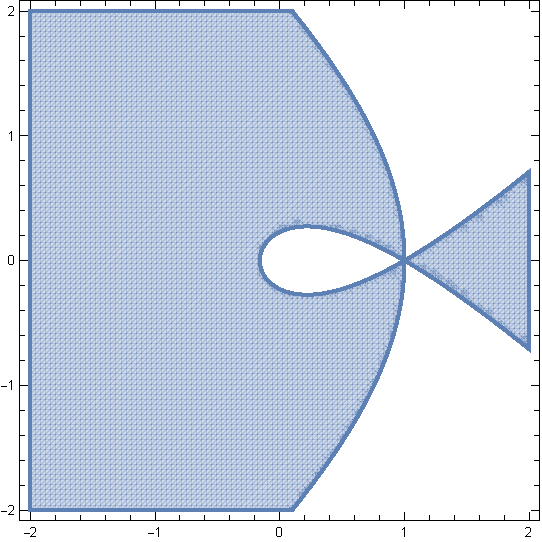
\includegraphics[height=.3\textwidth]{pictures/ReS_edge.pdf}
    \caption{The plot of the region $\operatorname{Re}S(z)-\operatorname{Re}S(1)>0$
			at the edge, in the neighborhood of the double critical point $w_c=1$.
			The new $w$ contour should pass through the shaded region,
		and the new $z$ must stay in the non-shaded region.}
    \label{fig:ReS_edge}
\end{figure}
Note however that the old $z$ contour must encircle $z=a$ and $z=0$,
and $z=a$ is a pole of the integrand. The $w$ contour must always be to the right of
the $z$ contour.

We see that there are three regimes, which we consider in the next three subsections.
\subsection{Airy kernel}
	If $a<1$, we can deform the $z$ contour to encircle $z=0$ and $z=a$,
		and the $w$ contour to pass through $w=1$. This will lead to the Airy kernel,
		and the derivation is the same as in
		\href{https://lpetrov.cc/rmt25/rmt25-notes/rmt2025-l07.pdf}{Lecture 7}.
		We obtain\footnote{Here and below, we understand the convergence
			of the kernels is up to a gauge transformation of the form
		$K(x,y)\mapsto\frac{f(x)}{f(y)}K(x,y)$.}
		\begin{equation*}
			z=1+\frac{Z}{n^{1/3}},\quad w=1+\frac{W}{n^{1/3}},\qquad
			x'=\frac{\xi}{n^{1/6}}, \quad y'=\frac{\eta}{n^{1/6}},
			\qquad
			\frac{1}{n^{1/6}}K_n\to K_{\mathrm{Airy}}(\xi,\eta).
		\end{equation*}
		Here
		\[
			K_{\mathrm{Airy}}(\xi,\eta)=
			\frac{1}{(2\pi i)^2}\iint \frac{\exp\left\{ \frac{W^3}{3}-\xi W-\frac{Z^3}{3}+\eta Z \right\}}{W-Z}\,dW\,dZ.
		\]
		Indeed, the only one new thing that happens here is that $a<1$, and so
		\begin{equation}
			\label{eq:z-w-extra-factor}
			\frac{w-a}{z-a}=\frac{1-a+W/n^{1/3}}{1-a+Z/n^{1/3}}=1+O(n^{-1/3}),
		\end{equation}
		so this term does not contribute to the asymptotics of the kernel.

\subsection{BBP transition and the deformed Airy kernel}

		If $a=1$, the behavior is going to be critical --- we still will
		be able to get the same scaling, but the limiting kernel will be different.
		Moreover, looking at \eqref{eq:z-w-extra-factor}, we see that
		we need to critically rescale $a$, so
		\begin{equation*}
			a=1+A n^{-1/3},
			\qquad
			\frac{w-a}{z-a}=\frac{W-A}{Z-A}+O(n^{-4/3}),
			\qquad
			\frac{1}{n^{1/6}}K_n\to \tilde K_{\mathrm{Airy}}(\xi,\eta),
		\end{equation*}
		where
		\begin{equation*}
			\tilde K_{\mathrm{Airy}}(\xi,\eta)=
			\frac{1}{(2\pi i)^2}\iint \frac{\exp\left\{
			\frac{W^3}{3}-\xi W-\frac{Z^3}{3}+\eta Z
			\right\}}{W-Z}
			\frac{W-A}{Z-A}
			\,dW\,dZ.
		\end{equation*}
		This kernel is the BBP transition kernel,
		first obtained in the seminal paper by
		Baik--Ben Arous--P\'ech\'e~\cite{BBP2005phase}.
		The spiked top eigenvalue distribution (and the Tracy--Widom distribution)
		are widely used in statistics of high-dimensional,
		highly correlated data.

\subsection{Gaussian regime}
\label{sec:gaussian-regime}

Finally, for $a>1$, we cannot deform the integration contours so that they
pass through the double critical point $w_c=1$.
Instead, we can make the contours pass through the point $a$ itself,
and scale the integration variables $w,z$ around $a$ on the scale $n^{-1/2}$ and
not $n^{-1/3}$.

Moreover, we need to make $x,y$ to scale around a different location
instead of $2\sqrt n$. We can find this location by first considering
$x=c\sqrt n$ and expanding as $n\to\infty$:
\begin{multline*}
	n\left( \frac{w^2}{2}-yw/\sqrt{n}+\log w \right)\Big\vert_{w=a+W/\sqrt n,\ y=c\sqrt n+\eta}\\=
	n \left(\frac{a^2}{2}-a c+\log (a)\right)+\sqrt{n} \left(-a \eta +a W+\frac{W}{a}-c W\right)-
	\frac{W^2}{2 a^2}+\frac{W^2}{2}-\eta  W.
\end{multline*}
The term by $n$ is the same in $S(w)$ and $S(z)$ and thus cancels out.
The term by $\sqrt n$ depends on $W$ and cannot be simply removed by a gauge transformation,
so we need to match $c$. We have
\begin{equation*}
	c=a+\frac{1}{a}.
\end{equation*}
\begin{remark}
	You can go to \url{https://lpetrov.cc/simulations/2025-01-28-bbp-transition/}
	and set the parameter $\theta$ (which is the same as $a$)
	to an integer, make $N$ large, and check that the location of the top or bottom eigenvalue
	becomes exactly $a+1/a$. (Despite the fact that the simulation at the link is for $\beta=1$.)
\end{remark}
Setting $c=a+1/a$, we have
\begin{equation*}
	n\ssp S\sim -\frac{W^2}{2 a^2}+\frac{W^2}{2}-\eta  W,
\end{equation*}
and thus the distribution of the top eigenvalue is given by
a Fredholm determinant with the kernel
\begin{equation*}
	K_G(\xi,\eta)=
	\frac{1}{(2\pi)^2}
	\int \int
	\exp\left\{
		\frac{a^{-2}-1}{2}(Z^2-W^2)-\eta W+\xi Z
	\right\}\cdot
	\frac{W}{Z}\cdot
	\frac{dW\,dZ}{W-Z}
\end{equation*}
Note that the factor $\sqrt n$ in front of $K_t$ is precisely
removed by the scaling of $w,z$, and there is no additional scaling
coming from the map $(x,y)\mapsto (\xi,\eta)$.
The contribution
from $(w-a)/(z-a)$ becomes $W/Z$.

The integration contours in $K_G$ are
such that $Re (W^2)>0$ and $Re (Z^2)<0$ on them, and this can be achieved by
the contour deformation.
Indeed, in the new variables, the
behavior at $W=Z=0$ is quadratic, so the
$Z$ contour must pass on the left, and the $W$ contour must be on the right.
One can check that this contour deformation is possible.

\begin{figure}[htpb]
    \centering
    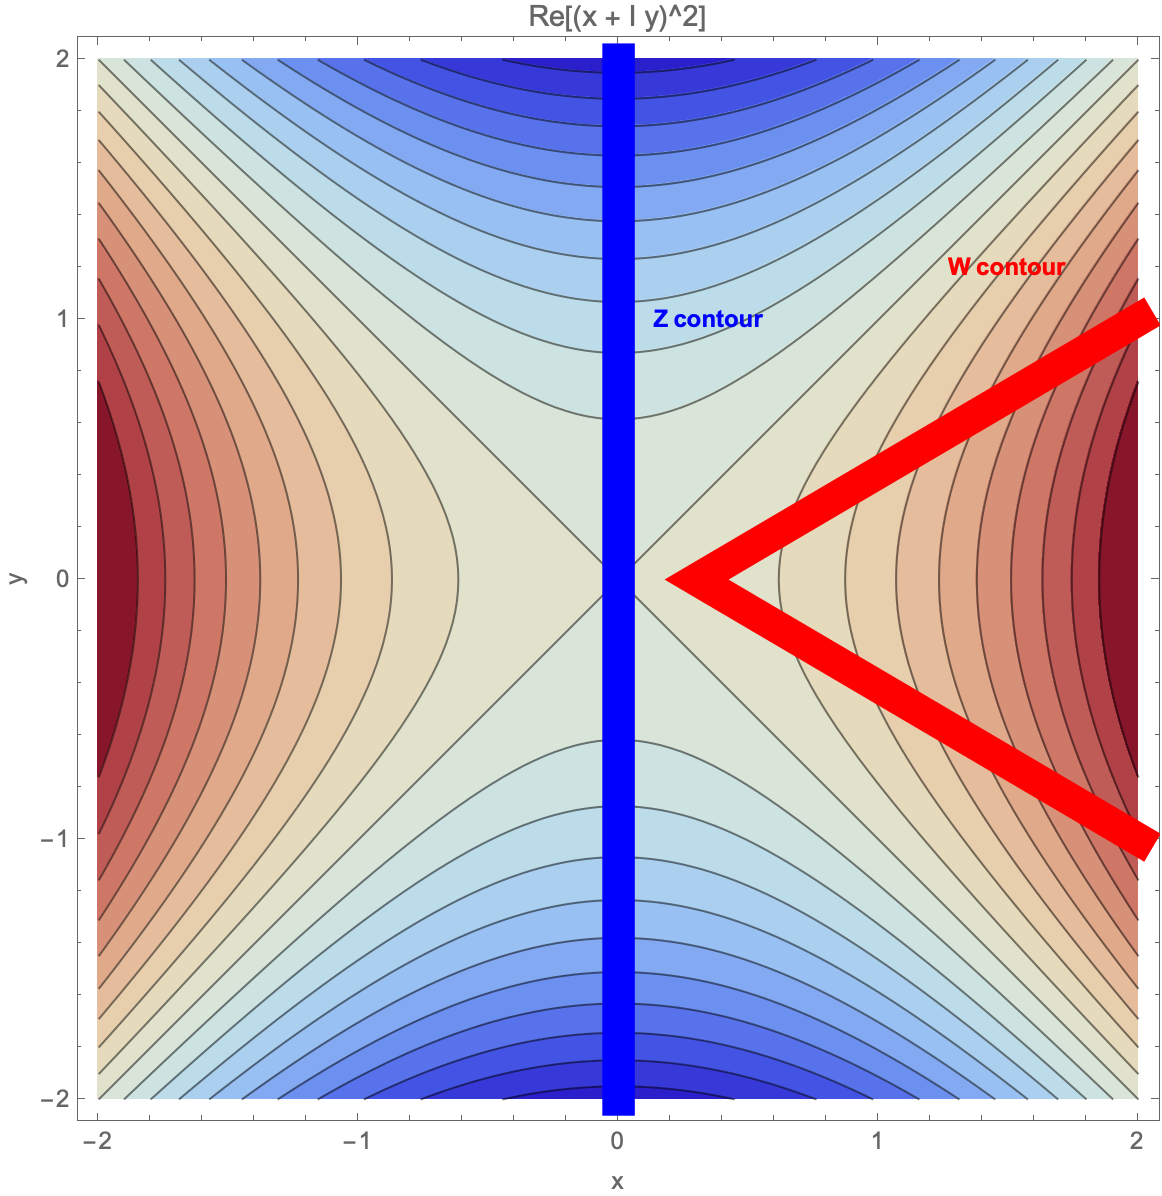
\includegraphics[height=.4\textwidth]{pictures/ReS_Gauss.png}
    \caption{The contour plot of
		$\Re(Z^2)$ around zero. Blue shades correspond to negative values, and yellow to positive. The
		$Z$ contour must pass through the blue region and becomes vertical, and the
		$W$ contour must stay in the yellow region, and becomes a union of two half-lines,
		which are at the angle $<\frac{\pi}{4}$ from the real line.}
		\label{fig:ReS_Gauss}
\end{figure}

\subsection{Matching Fredholm determinant to the Gaussian distribution}

Let us renormalize the integration variables
to remove the factor $a^{-2}-1$ in front of the squares,
and match $\det\left( 1-K_G \right)_{\ge x}$ to the Gaussian distribution
(see also Problem~\ref{prob:GUE-kernel} for another way to match).
We will work with
\begin{equation*}
	K_G(\xi,\eta)=
	\frac{1}{(2\pi)^2}
	\int \int
	\exp\left\{
		\frac{1}{2}(Z^2-W^2)-\eta W+\xi Z
	\right\}\cdot
	\frac{W}{Z}\cdot
	\frac{dW\,dZ}{W-Z}
\end{equation*}
The discussion below is informal, but can be easily made rigorous.

\medskip

\noindent\textbf{Step 1. Partial fractions and decomposition.}
Observe that
\[
\frac{W}{Z(W-Z)} \;=\;
\frac{1}{Z}\;+\;\frac{1}{\,W-Z\,}.
\]
Thus we can write
\[
K_G(\xi,\eta)
=
K^{(1)}(\xi,\eta)+K^{(2)}(\xi,\eta),
\]
where
\begin{align*}
K^{(1)}(\xi,\eta)
&=
\frac{1}{(2\pi)^2}
\int\!\int
\exp\!\Bigl(\tfrac12(Z^2-W^2)+\xi Z-\eta W\Bigr)\,\frac{1}{Z}\,dW\,dZ,
\\
K^{(2)}(\xi,\eta)
&=
\frac{1}{(2\pi)^2}
\int\!\int
\exp\!\Bigl(\tfrac12(Z^2-W^2)+\xi Z-\eta W\Bigr)\,\frac{1}{W-Z}\,dW\,dZ.
\end{align*}
The term $K^{(1)}$ has a factor $\frac{1}{Z}$ independent of $W-Z$,
while $K^{(2)}$ contains the remaining part $\frac{1}{\,W-Z\,}$.

\medskip

\noindent\textbf{Step 2. Analysis of $K^{(1)}$.}
Focus on
\[
K^{(1)}(\xi,\eta)
=
\frac{1}{(2\pi)^2}
\Bigl(\int
e^{\frac12Z^2+\xi Z}\,\frac{dZ}{Z}\Bigr)
\Bigl(\int
e^{-\frac12W^2-\eta W}\,dW\Bigr).
\]
The operator $K^{(1)}$ is a rank-1 operator in the variables $\xi,\eta$:
\[
K^{(1)}(\xi,\eta)
=
u(\xi)\,v(\eta)
\]
for some functions $u(\cdot)$ and $v(\cdot)$ of one variable each.
Hence $K^{(1)}$ has at most one nonzero eigenvalue (its trace).

\medskip

\noindent\textbf{Step 3. Representation of $K^{(2)}$ and the key identity.}
For $K^{(2)}$, we use
\[
\frac{1}{\,W-Z\,}=\int_0^{\infty} e^{-t(W-Z)}\,dt
\]
(again justified by the choice of integration contours). Then
\[
K^{(2)}(\xi,\eta)
=
\int_0^\infty
\Bigl[
\frac{1}{2\pi i}\!\int
e^{\frac12Z^2+(\xi+t)Z}\,dZ
\Bigr]
\Bigl[
\frac{1}{2\pi i}\!\int
e^{-\frac12W^2-(\eta+t)W}\,dW
\Bigr]dt.
\]
Denote
\[
A(\xi,t)
=
\frac{1}{2\pi i}\int
e^{\frac12Z^2+(\xi+t)Z}\,dZ,
\quad
B(t,\eta)
=
\frac{1}{2\pi i}\int
e^{-\tfrac12W^2-(\eta+t)W}\,dW.
\]
Hence
\(
K^{(2)}(\xi,\eta)=\int_0^\infty A(\xi,t)\,B(t,\eta)\,dt.
\)
In operator form on suitable spaces,
this reads $K^{(2)}=A\,B$, and one checks $B\,A=I$
(\emph{identity on the $t$-variable space}),
so $A\,B$ and $B\,A$ share the same nonzero spectrum.
Indeed,
\begin{equation*}
	BA(s,t)=\frac{1}{(2\pi i)^2}
	\int_{\mathbb{R}}d\xi
	\int dW\, dZ
	e^{-\frac{1}{2}W^2+\frac{1}{2}Z^2}
	e^{-(s+\xi)W+(\xi+t)Z}.
\end{equation*}
Integrating over $\xi$ in the Fourier sense yields the delta:
\begin{equation*}
	\int_{\mathbb{R}}d\xi e^{\xi(Z-W)}=2\pi\delta(Z-W).
\end{equation*}
Integrating in $W$ is again an integral of $e^{(t-s)W}$, and thus, the second $2\pi$ disappears,
and we arrive at $BA(s,t)=\delta(s-t)$, which is the kernel of the identity operator.

We conclude that $AB$ is a projection, since
$(AB)^2=ABAB=AB$.

\medskip
\noindent\textbf{Step 4. Conclusion.}
We then have
\begin{equation*}
	\det\left( 1-K_G \right)_{\ge x}=\det(I-K^{(1)}-K^{(2)})_{\ge x}.
\end{equation*}
The operators $K^{(1)}$ and $K^{(2)}$ have a special structure. As shown above, $K^{(2)}=AB$ is a projection operator, satisfying $(K^{(2)})^2=K^{(2)}$. This means its eigenvalues are either 0 or 1, corresponding to the inactive and active subspaces, respectively. Let $\mathcal{V}=\mathrm{Ran}(B)$ be the active subspace.

Meanwhile, $K^{(1)}$ is a rank-1 operator, which we can write as $K^{(1)}=u\otimes v$ for some functions $u,v$ (as already defined above). One can verify that the range of $K^{(1)}$ is contained in $\mathcal{V}$, meaning that $K^{(1)}$ maps into the same subspace where $K^{(2)}$ acts as identity.

The full operator $I-K_G$ differs from identity only in a one-dimensional subspace. To compute the Fredholm determinant, we need only the one non-trivial eigenvalue, which comes from the action of $K_G$ on the direction of $u$ within $\mathcal{V}$. This eigenvalue equals the trace, $\lambda_{\text{special}}=\langle v,u\rangle$.
Therefore, the Fredholm determinant reduces to:
\begin{equation*}
	\det\left(1-K_G\right)_{\ge x}=(1-\lambda_{\text{special}})=(1-\langle v,u\rangle).
\end{equation*}

Direct computation of this inner product, using the explicit forms of $u$ and $v$ from the partial fraction decomposition, yields:
\begin{equation*}
	\langle v,u\rangle=\int_{x}^{\infty}v(w)u(w)\,dw=1-\Phi(x),
\end{equation*}
where $\Phi(x)$ is the standard Gaussian cumulative distribution function.

This gives us the final result:
\begin{equation*}
	\det\left(1-K_G\right)_{\ge x}=(1-(1-\Phi(x)))=\Phi(x).
\end{equation*}

Thus, the Fredholm determinant exactly matches the Gaussian CDF, confirming that the distribution of the outlier eigenvalue in the $a>1$ regime is precisely Gaussian.


\section{Airy line ensemble}



\begin{theorem}[Edge scaling limit to Airy line ensemble]
	Consider an $N\times N$ GUE (Gaussian Unitary Ensemble) Dyson Brownian motion, i.e., the stochastic process of eigenvalues $(\lambda_1(t)\ge \cdots\ge \lambda_N(t))_{t\in\mathbb{R}}$ evolving under Dyson's eigenvalue dynamics. After centering at the spectral edge parallel to the vector $\mathbf{v}_t$ and applying the
Airy scaling (tangent axis scaled by $N^{-1/3}$ and fluctuations scaled by $N^{-1/6}$), the top $k$ eigenvalue trajectories converge as $N\to\infty$ to the \textbf{Airy line ensemble}. In particular, for each fixed $k\ge1$ the rescaled process $$(N^{1/6}[\lambda_i(\langle
			N^{-1/3},N^{-1/6}
\rangle \cdot \mathbf{v})-c_{N,t}])_{1\le i\le k}$$ converges in distribution (uniformly on compact $t$-intervals) to $(\mathcal{P}_i(t))_{1\le i\le k}$, where $\{\mathcal{P}_i(t)\}_{i\ge1}$ is the parabolic Airy line ensemble. Consequently, the top curve $\mathcal{L}_1(t)$ is the \textbf{Airy$_2$ process}, which is the $t$-stationary scaling limit of the largest eigenvalue process.
\end{theorem}

Let us define $\mathcal{L}_i(t)=\mathcal{P}_i(t)+t^2$, and call $\mathcal{L}$ the Airy Line Ensemble
(without the word ``parabolic''). One can (correctly) think that the parabola comes
from the scaling window, which is of different proportions in the horizontal and vertical directions.

\begin{theorem}[Airy line ensemble is Brownian Gibbsian \cite{CorwinHammond2013}]
The parabolic Airy line ensemble $\{\mathcal{P}_i(t)\}_{i\ge1}$ satisfies the \textbf{Brownian Gibbs property}. Namely, for any fixed index $k\ge1$ and any finite time interval $[a,b]$, conditioning on the outside portions of the ensemble (i.e., $\{\mathcal{P}_j(t): t\notin[a,b]\}$ for all $j$, and $\{\mathcal{P}_j(t): j\neq k\}$ for $t\in[a,b]$), the conditional law of the $k$th curve on $[a,b]$ is that of a \textbf{Brownian bridge} from $(a,\mathcal{P}_k(a))$ to $(b,\mathcal{P}_k(b))$ \textbf{conditioned} to stay above the $(k+1)$th curve and below the $(k-1)$th curve on $[a,b]$. In particular, the Airy line ensemble is invariant under this resampling of a single curve by a conditioned Brownian bridge.
\end{theorem}

At the same time, the Airy line ensemble $\mathcal{L}$ is time-stationary.

\begin{theorem}[Unique characterization of ALE \cite{AggarwalHuang2023Characterization}]
	The parabolic Airy line ensemble is the \textbf{unique} Brownian Gibbs line ensemble satisfying a natural parabolic curvature condition on the top curve. More precisely, let $\boldsymbol{\mathcal{P}}=(\mathcal{P}_1,\mathcal{P}_2,\ldots)$ be any line ensemble that satisfies the Brownian Gibbs property. Suppose in addition that the top line $\mathcal{P}_1(t)$ \textbf{approaches a parabola} of curvature $1/\sqrt{2}$ at infinity. Then $\boldsymbol{\mathcal{L}}$ must coincide (in law) with the \textbf{parabolic Airy line ensemble}, up to an overall affine shift of the entire ensemble.
\end{theorem}




\appendix
\setcounter{section}{10}

\section{Problems (due 2025-04-29)}


\subsection{Biorthogonal ensembles}
\label{prob:biorthogonal}

Derive \Cref{thm:dbm-det-kernel} from
\Cref{lem:density_representation}
using the orthogonalization process similar
to~\href{https://lpetrov.cc/rmt25/rmt25-notes/rmt2025-l05.pdf}{Lecture 5},
and then taking the limit as $s\to\infty$.

\subsection{Scaling of the kernel}
\label{prob:scaling}

Let $a_i=0$ in \Cref{thm:dbm-det-kernel}.
Find $\alpha$ such that
$t^\alpha K_t(x/\sqrt{t},y/\sqrt{t})$ is independent of $t$.
Can you explain this value of $\alpha$?

\subsection{Gaussian regime and integration contours}

Check that the contour deformation
from $(z,w)$ to $(Z,W)$ passing through $a$
described in
\Cref{sec:gaussian-regime} is valid.

\subsection{GUE kernel}
\label{prob:GUE-kernel}

Consider the following generalization of the kernel $K_G$
from \Cref{sec:gaussian-regime}:
\begin{equation*}
	K_G^m(\xi,\eta)=
	\frac{1}{(2\pi)^2}
	\int \int
	\exp\left\{
		\frac{1}{2}(Z^2-W^2)-\eta W+\xi Z
	\right\}\cdot
	\left(
	\frac{W}{Z}
\right)^{m}
\frac{dW\,dZ}{W-Z},
\end{equation*}
where $m\ge1$ is an integer and the contours are as in \Cref{fig:ReS_Gauss}.
Show that the Fredholm determinant
$\det\left( 1-K_G^m \right)_{L^2(x,+\infty)}$
is the cumulative distribution function of the largest eigenvalue
of the $m\times m$ GUE matrix.



\bibliographystyle{alpha}
\bibliography{bib}


\medskip

\textsc{L. Petrov, University of Virginia, Department of Mathematics, 141 Cabell Drive, Kerchof Hall, P.O. Box 400137, Charlottesville, VA 22904, USA}

E-mail: \texttt{lenia.petrov@gmail.com}


\end{document}
